\subsection{Exemple d'utilisation de Claude}

\begin{bfbox}{La création des \frquote{\textsc{toolbox}}}

    Pour fournir les kits d'outils des exercices de cette formation, j'ai demandé à Claude code de me préparer des designs dont je pourrais m'inspirer. 

    J'ai utilisé l'agent scripteur décrit dans cette formation. 

    \begin{tcbenumerate}[2]
        \tcbitem \acc{Le prompt}. \mycomment{On ne s'est pas appliqué. C'est possible grâce à la qualité du pré-prompt.}
        \begin{center}
        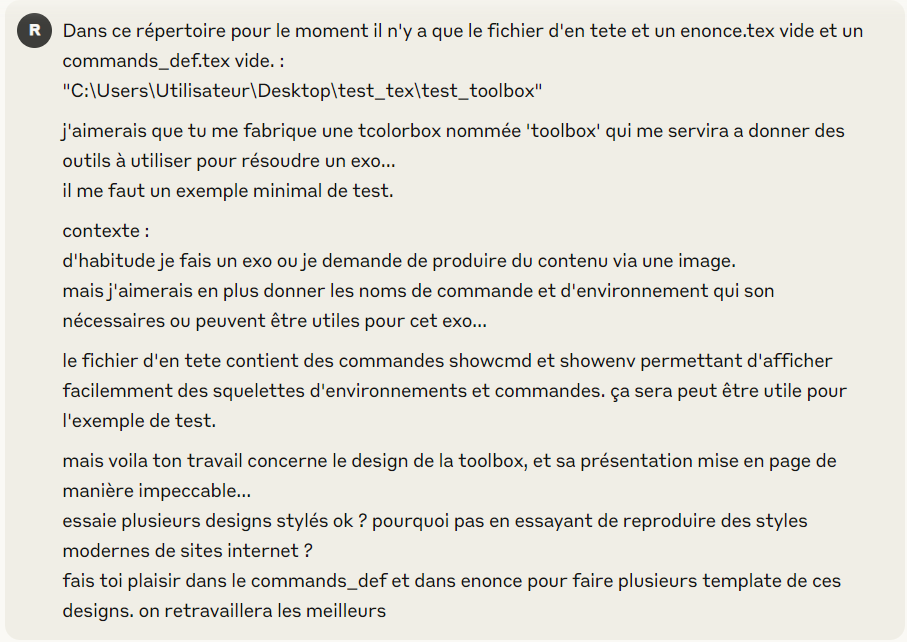
\includegraphics[width=0.75\textwidth]{annexes/Example_craft_toolbox/1.png}
        \end{center}
        
        \tcbitem \acc{L'action'}. \mycomment{Le modèle analyse le contenu, puis agis. Il tente même de compiler avec plusieurs compilateurs.}
        \begin{center}
        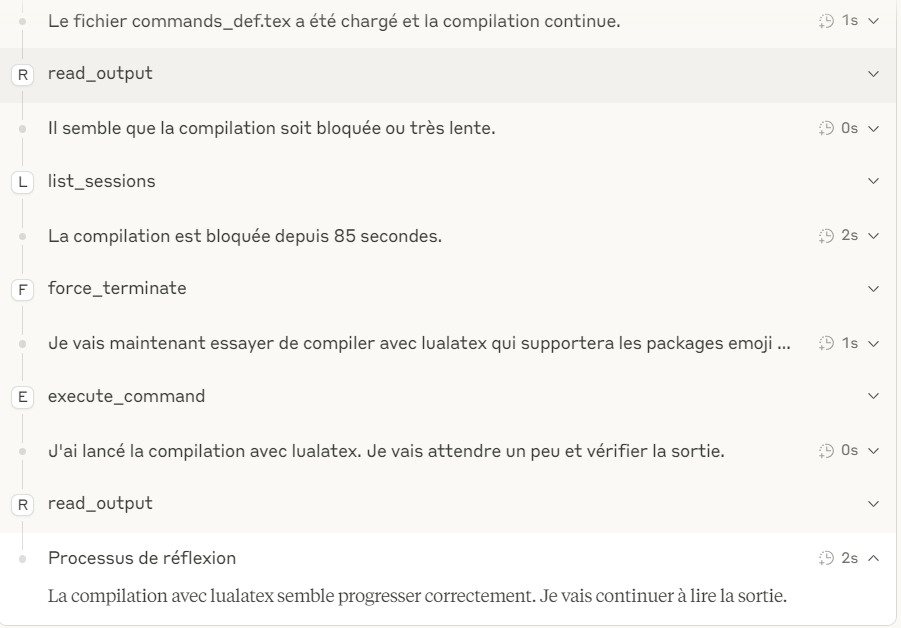
\includegraphics[width=0.75\textwidth]{annexes/Example_craft_toolbox/3.png}
        \end{center}

        \tcbitem \acc{Le rendu}. \mycomment{Claude a été efficace, je n'ai plus qu'à choisir parmi les $8$ exemples fournis.}
        \begin{center}
        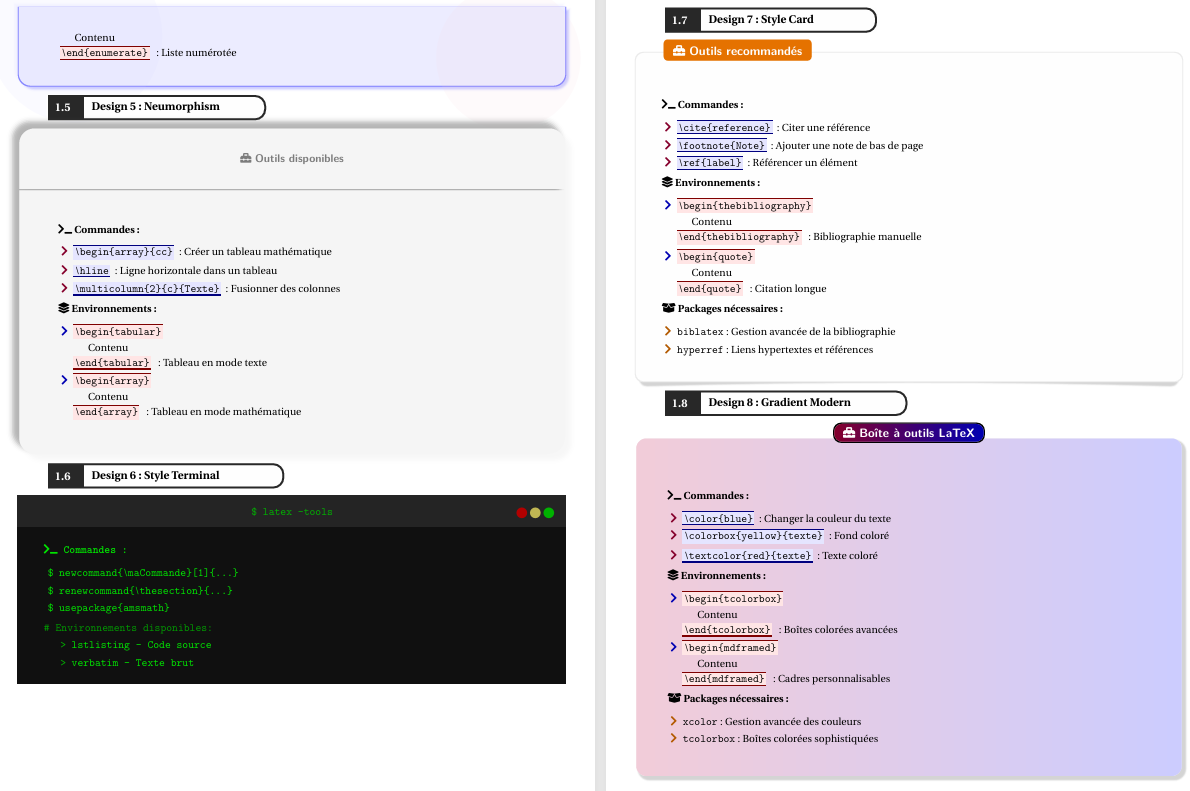
\includegraphics[width=0.75\textwidth]{annexes/Example_craft_toolbox/4.png}
        \end{center}     
        
        \tcbitem \acc{L'investissement en temps} :

        En regardant les propriétés du dossier de test pour ces exemples de design, on a :  
        \begin{itemize}[label=$\bullet$]
            \item \encadrer{Date de création : 8h23}
        
            \item \encadrer[green]{Date de fin d'édition de cet exemple : 9h}
        \end{itemize}

        La création de cet exemple et du design des mes \textsc{toolbox} n'a pris qu'un peu plus d'une demi-heure.
    \end{tcbenumerate}
\end{bfbox}